\documentclass[12pt]{article}
\usepackage[margin=0.5in]{geometry}                % See geometry.pdf to learn the layout options. There are lots.
\geometry{letterpaper} 
                  % ... or a4paper or a5paper or ... 
%\geometry{landscape}                % Activate for for rotated page geometry
%\usepackage[parfill]{parskip}    % Activate to begin paragraphs with an empty line rather than an indent
\usepackage{graphicx}
\usepackage{amssymb}
\usepackage{epstopdf}
\usepackage{hyperref}
\hypersetup{colorlinks,urlcolor=blue}

\DeclareGraphicsRule{.tif}{png}{.png}{`convert #1 `dirname #1`/`basename #1 .tif`.png}

%\graphicspath{{'../Figures/Data_cleaning_report/'}}

\title{PPOL 563 Data Visualization \\
Data collection \& cleaning report}
\author{Chau Nguyen}
\date{\today}                                           % Activate to display a given date or no date

\begin{document}


\maketitle

\textbf{Source:}
For this report, I am working with the \href{https://opendata.dc.gov/datasets/DCGIS::liquor-licenses/about}{Liquor Licenses dataset from DC Open Data}. \\

\textbf{License:}
The data is under Creative Commons CC BY 4.0, meaning I am free to share, copy and redistribute if in any medium or format, as well as adapt, transform and build upon it for any purposes as long as I give appropriate credit, provide a link to the license, and indicate if changes were made\footnote{ Source: \url{https://creativecommons.org/licenses/by/4.0/}}. \\

\textbf{Collection method:} I downloaded the data. The dataset was created by the DC Geographic Information System (DC GIS) for the DC Office of the Chief Technology Officer (OCTO). The Alcoholic Beverage Regulation Administration (ABRA) provided DC GIS staff with a database identifying locations and attributes of liquor licensees in DC. The DC GIS staff geo-processed the data. \\

\textbf{Biases and sampling:} I do not expect biases or sampling issues with this dataset, because it's a simply a descriptive dataset listing liquor licensees in Washington DC. The raw data contains 2,130 observations and 32 rows. \\

\textbf{Data Cleaning Methods \& Identified Issues:} I first used the missingno package to identify rows with missing numbers in my dataset. Figure \ref{missing} shows the features included in the dataset, as well as the missingness in each column. At first glance, I looks like the columns STORAGEFACILITY, DISTILLERY\_PUB and SPORTS\_WAGGERING contain all missing values.

\begin{figure}[h!]
\centering
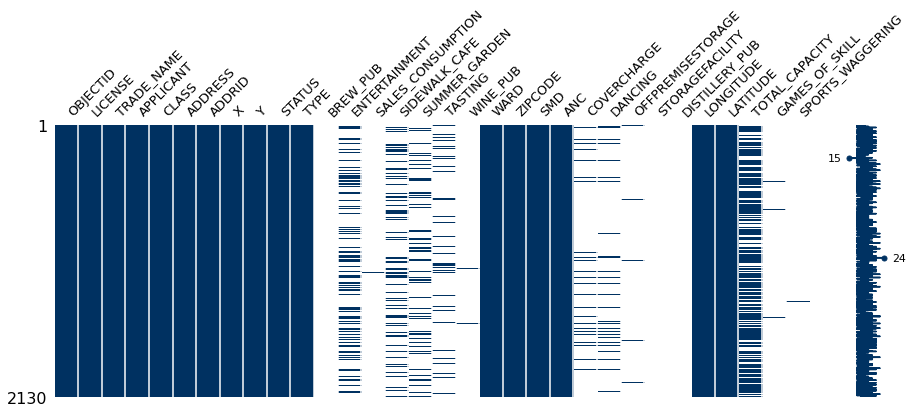
\includegraphics[width = 0.75\textwidth]{../Figures/Data_cleaning_report/missing_no.png}
\caption{Missingno matrix for DC Liquor Licensees dataset}
\label{missing}
\end{figure}

Figures \ref{missing} also tells me that many of the features indicating what type of establishments the liquor lincensee is such as BREW\_PUB and SIDEWALK\_CAFE should be re-coded as binary or boolean (the current values are ``nan'' and ``CHECKED'').


\begin{figure}[h!]
\centering
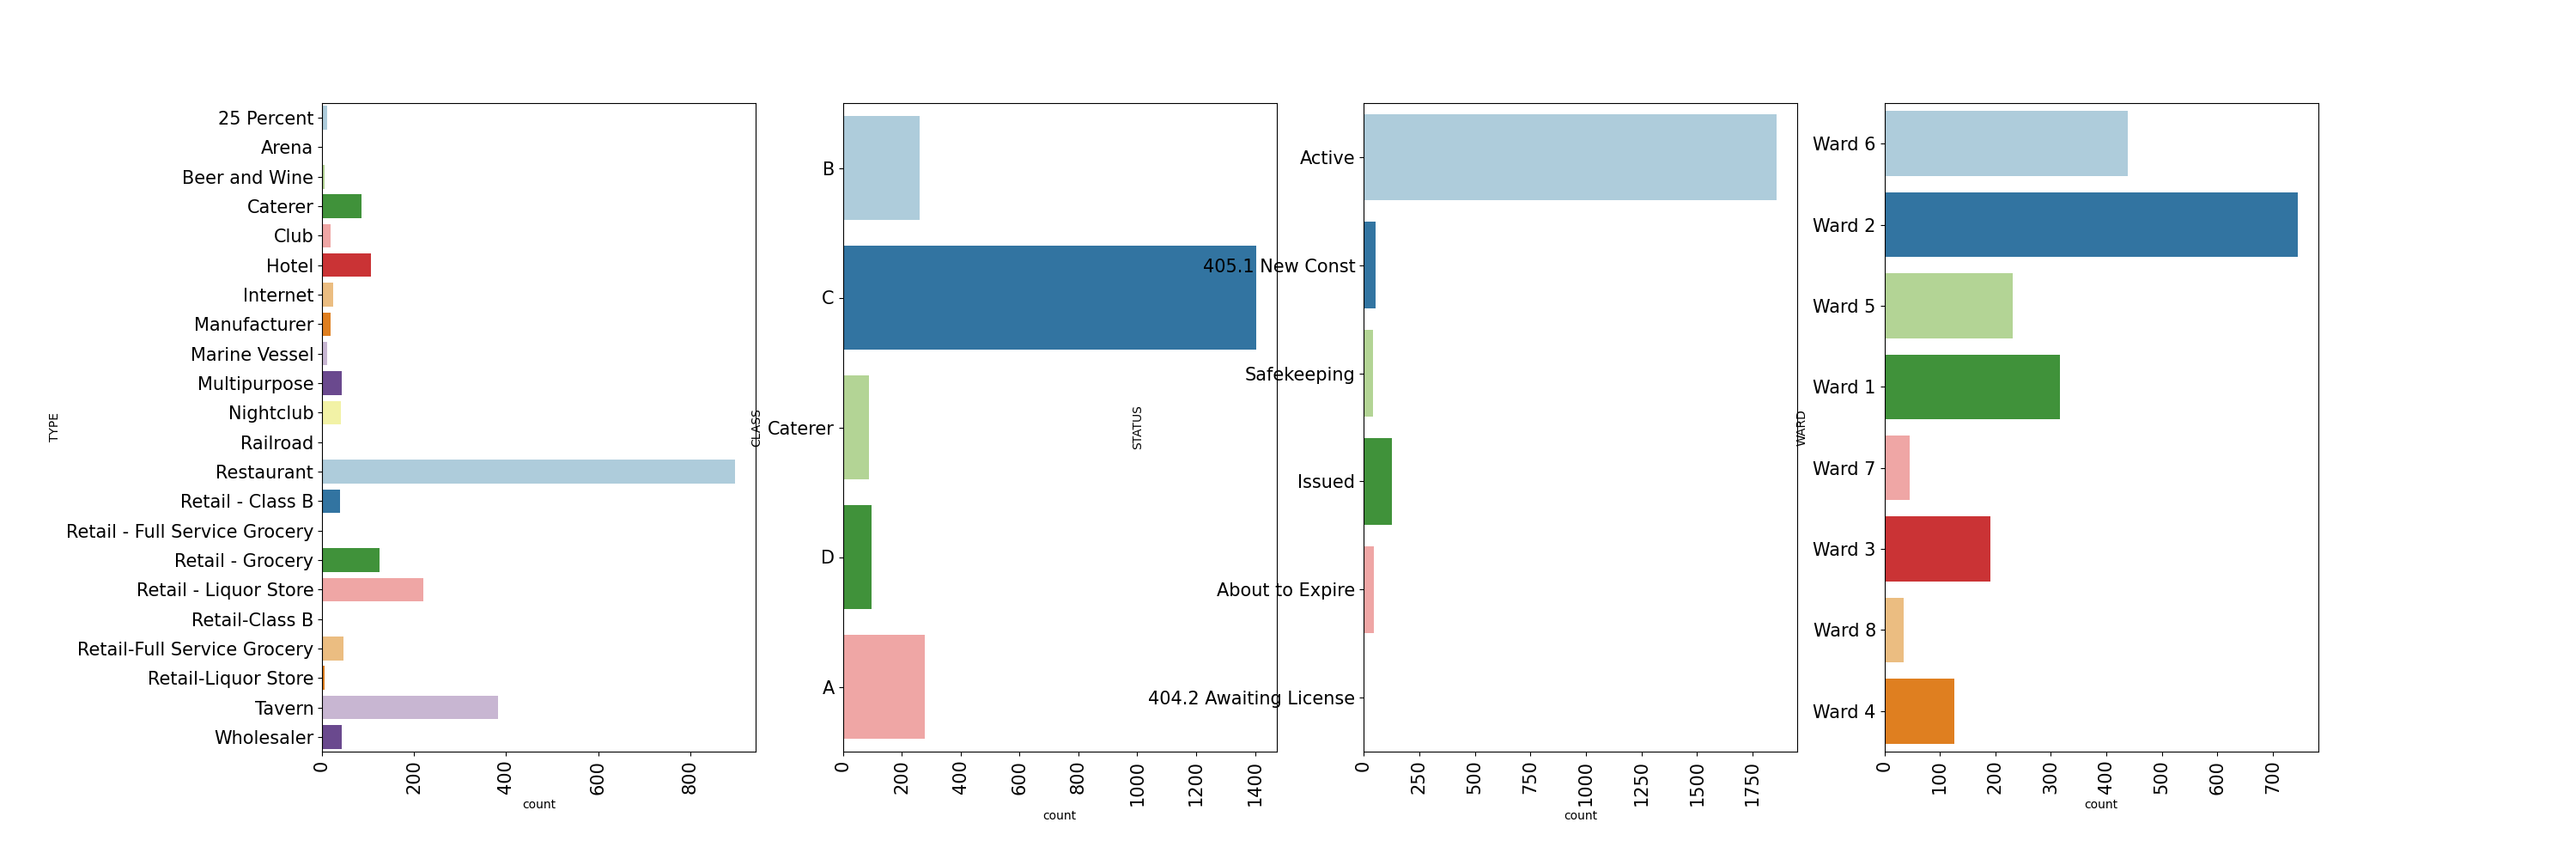
\includegraphics[width = \textwidth]{../Figures/Data_cleaning_report/cat.png}
\caption{Categorical data}
\label{cat}
\end{figure}
 
Figure \ref{cat} shows the number of observations for 4 categorical variables. From the left-most plot, we can see identify several issues with categories in the TYPE column: for example, ``Retail - Full Service Grocery" and ``Retail-Full Service Grocery" and ``Retail - Full Service Grocery" or ``Retail-Class B" and "Retail - Class B" are different categories due to the strings not matching.

A challenge with this dataset is that the \href{https://www.arcgis.com/sharing/rest/content/items/cabe9dcef0b344518c7fae1a3def7de1/info/metadata/metadata.xml?format=default&output=html}{metadata from Open DC} does not tell me what the categories should be or their definitions, but refer questions to the Alcoholic Beverage Regulation Administration (ABRA) who \href{https://abra.dc.gov/page/types-abc-licenses}{does not a great job in differentiating the categories either.} For now, I decided to keep ``Catering" as a license class in addition to A, B, C, D, leave the categories for status as is, and recoded the Wards as integers instead of string. I also found 13 instances where LICENSE was duplicated across columns. After checking the duplicated license numbers, I decided it was ok to only keep the last row in case of duplication\footnote{There were 6 licenses with 1 duplicate and 1 license with 2 duplicates - Gallaudet College. After checking, 2 of the duplicates for Gallaudet have the wrong street address - 700 Florida Ave NE when it should be 800. I kept the observation with the correct street address.}. After cleaning, the dataset has 2,123 rows and no missing data for the binary variables.

Figure \ref{missing} also shows me that there are many liquor licensees in Washington with missing capacity data. I wanted to check the distribution of the available data without dropping rows with missing values, so I created a histogram for log(TOTAL\_CAPACITY + 1) in figure \ref{log_cap}. Total capacity for observations where data is available seem to follow a normal distribution. 

\begin{figure}
\centering
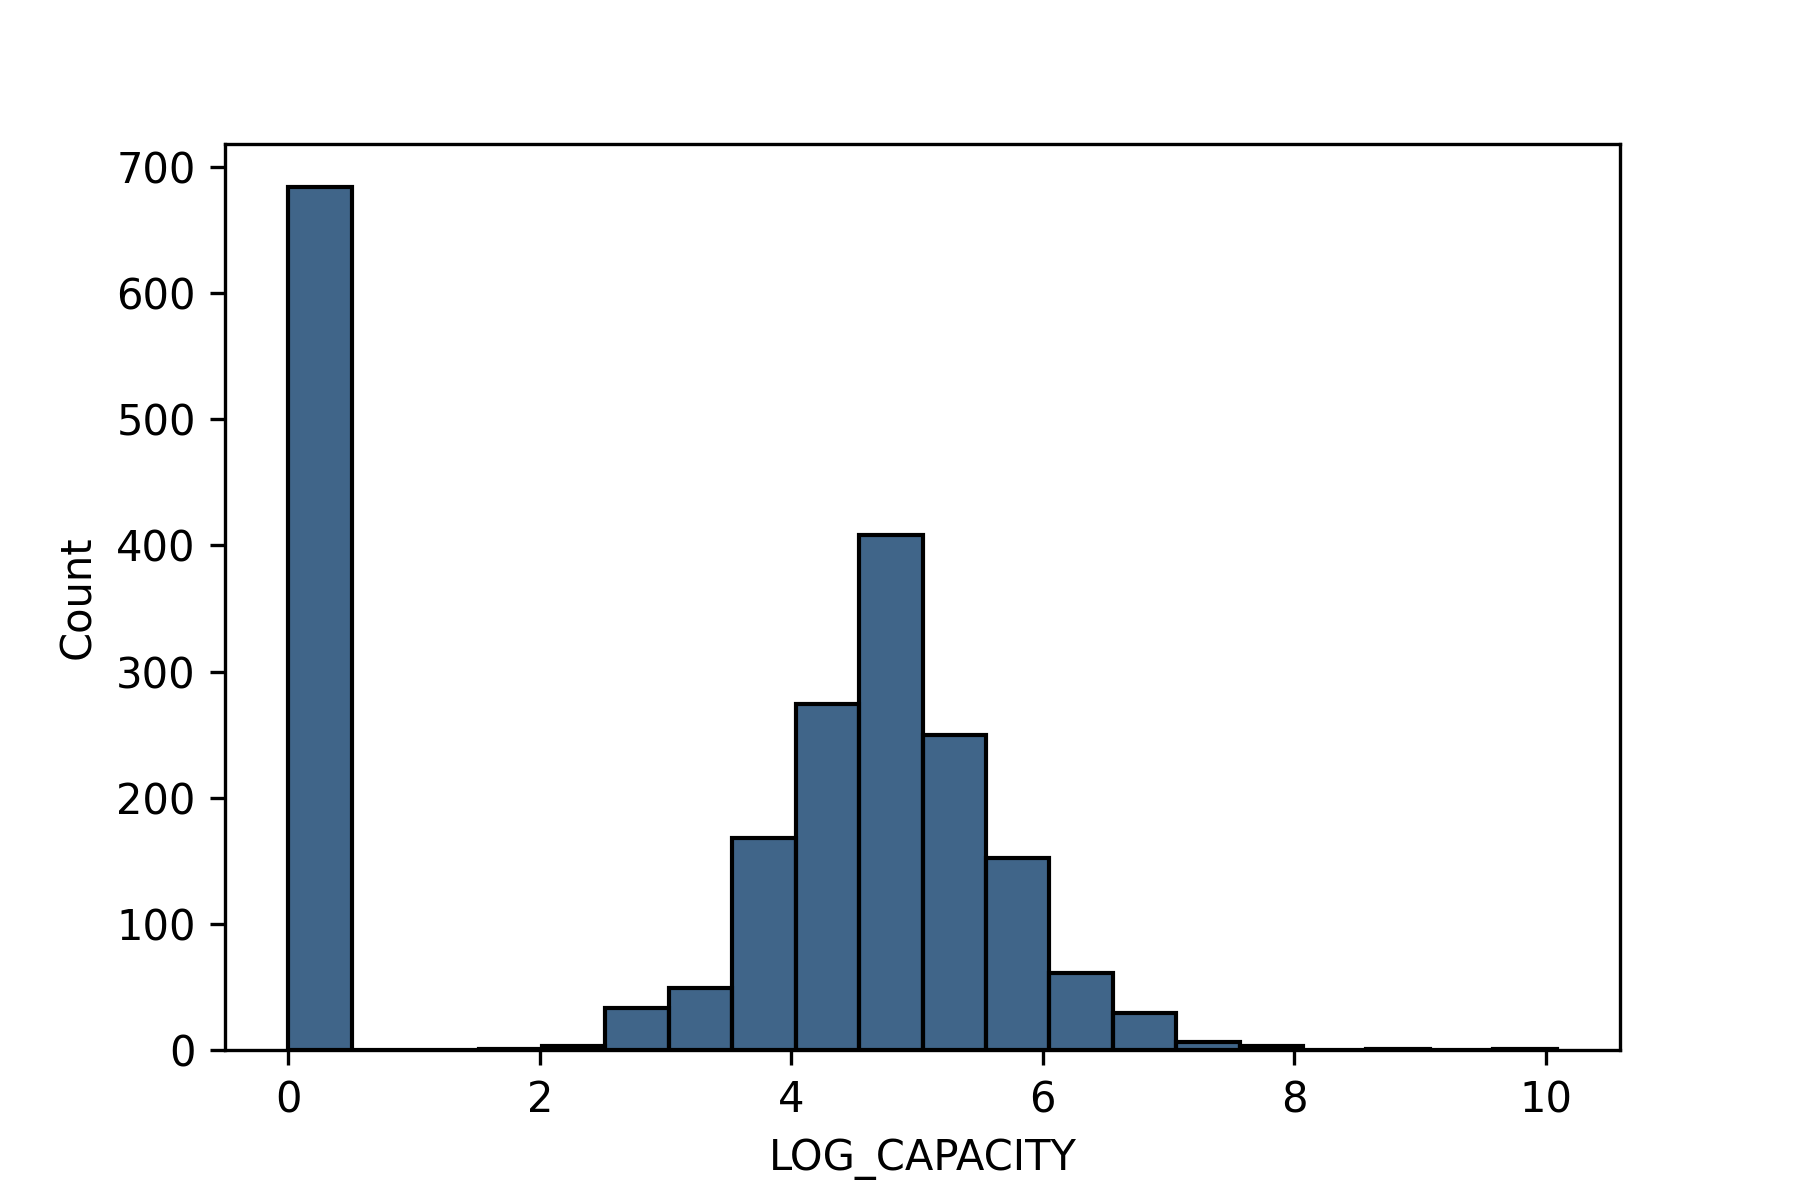
\includegraphics[width = 0.45\textwidth]{../Figures/Data_cleaning_report/log_capacity_missing.png}
\caption{Histogram for log capacity of liquor licensees in DC}
\label{log_cap}
\end{figure}


\subsubsection*{Data Dictionary of Key Features}

For this dataset, the important features can be grouped into several categories:

\begin{itemize}
	\item \textbf{Identifiers:}
		\subitem LICENSE: ABRA License 
	\item \textbf{Characteristics - categorical:}
		\subitem CLASS: License class
		\subitem STATUS: License status
		\subitem TYPE: Establishment type

	\item \textbf{Characteristics - numerical:}
		\subitem TOTAL\_CAPACITY: Establishment capacity
		
	\item \textbf{Location:}
		\subitem WARD
		\subitem ZIPCODE
		\subitem LONGITUDE
		\subitem LATITUDE
\end{itemize}

\begin{figure}[h!]
\centering
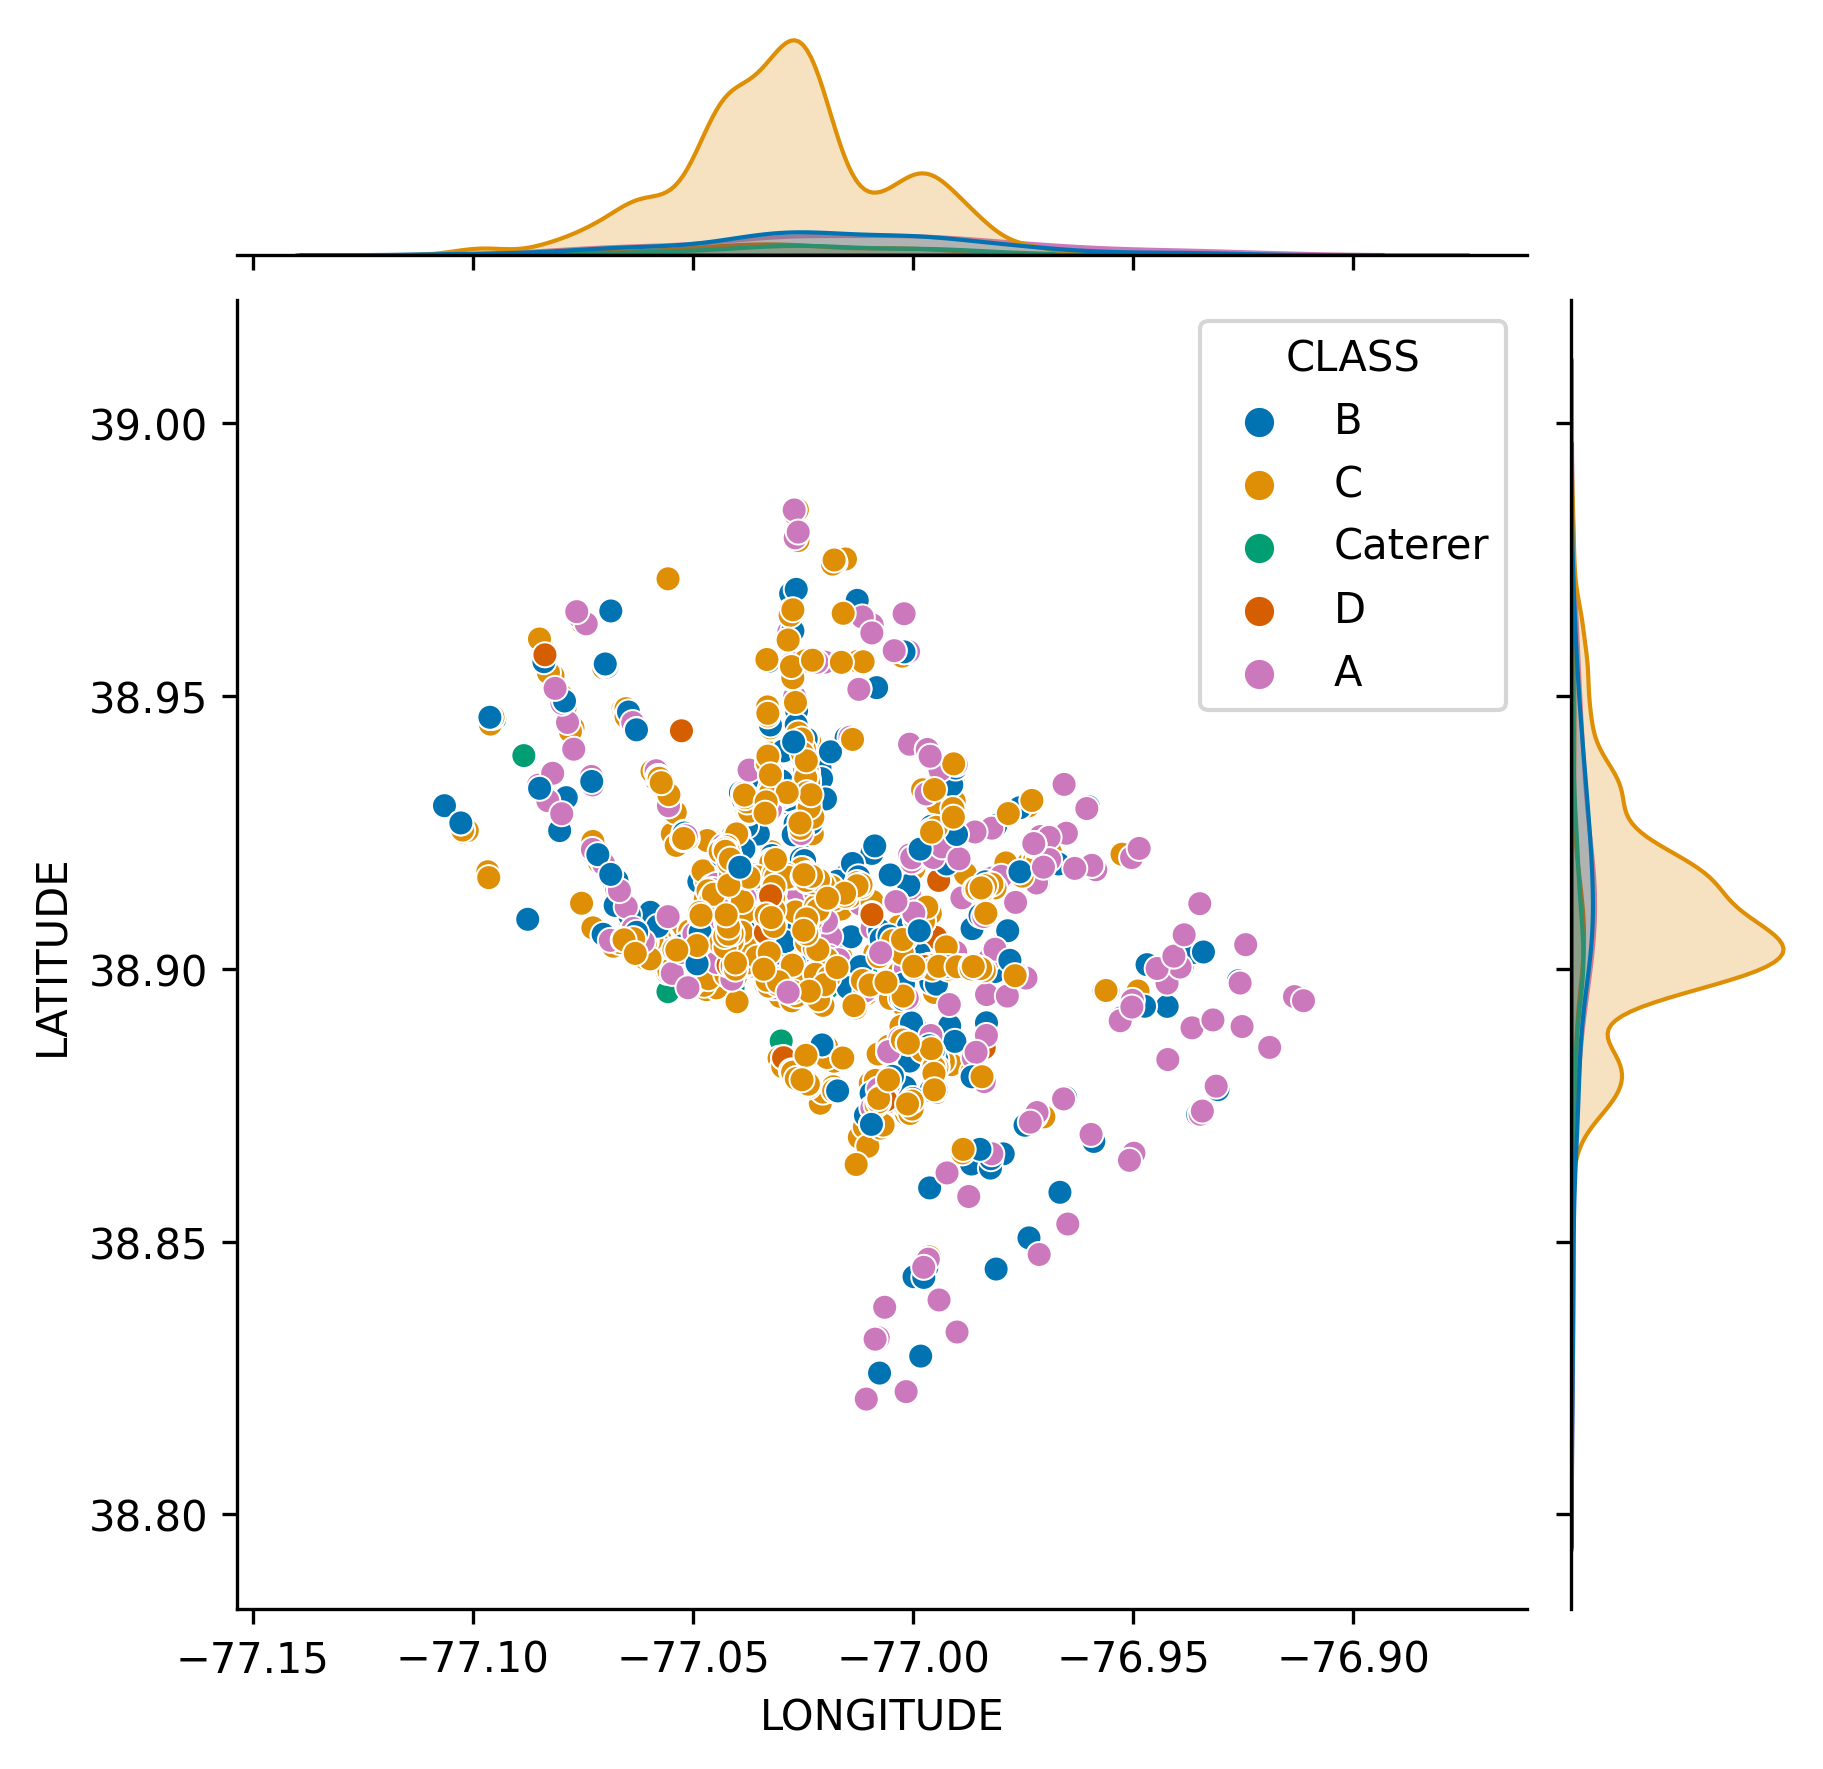
\includegraphics[width = 0.45\textwidth]{../Figures/Data_cleaning_report/long_lat.png}
\caption{DC Liquor Licensees}
\label{log_cap}
\end{figure}

This dataset itself can then be merged with different datasets such as Census Tract data for income and unemployment, DC crime maps, shapefiles for Ward and DC neighborhoods. I hope to be able to create different maps of DC neighborhoods \& wards in relations to the kind of establishments in each clusters.





\end{document}